\documentclass[12pt,UTF8]{ctexart}
\usepackage{ctex,amsmath,amssymb,geometry,fancyhdr,bm,amsfonts,mathtools,extarrows,graphicx,url,enumerate,xcolor,float,multicol,wasysym}
\usepackage{subfigure}

\allowdisplaybreaks[4]
% 加入中文支持
\newcommand\Set[2]{\left\{#1\ \middle\vert\ #2 \right\}}
\newcommand\Lim[0]{\lim\limits_{n\rightarrow\infty}}
\newcommand\LIM[2]{\lim\limits_{#1\rightarrow#2}}
\newcommand\Ser[1]{\sum_{n=#1}^\infty}
\newcommand{\SER}[2]{\sum_{#1=#2}^\infty}
\newcommand{\Int}[4]{\varint\nolimits_{#1}^{#2}#3\mathrm d#4}
\newcommand{\aIInt}[1]{\iint\limits_{#1}}
\newcommand{\IInt}[3]{\iint\limits_{#1}#2\mathrm d#3}
\newcommand{\varIInt}[4]{\iint\limits_{#1}#2\mathrm d#3\mathrm d#4}
\newcommand{\IIInt}[3]{\iiint\limits_{#1}#2\mathrm d#3}
\newcommand{\varIIInt}[5]{\iiint\limits_{#1}#2\mathrm d#3\mathrm d#4\mathrm d#5}
\newcommand{\LInt}[3]{\varint\nolimits_{#1}#2\mathrm d#3}
\newcommand{\LOInt}[3]{\varoint\nolimits_{#1}#2\mathrm d#3}
\newcommand{\LLInt}[4]{\varint\nolimits_{#1}\nolimits^{#2}#3\mathrm d#4}
\newcommand{\BLInt}[2]{\varint\nolimits_{#1}#2}
\newcommand{\varBLInt}[3]{\varint\nolimits_{#1}\nolimits^{#2}#3}
\newcommand{\BLOInt}[2]{\varoint\nolimits_{#1}#2}
\newcommand{\SIInt}[3]{\iint\limits_{#1}#2\mathrm d#3}
\newcommand{\md}[1]{\mathrm d#1}
\newcommand{\BSIInt}[2]{\iint\limits_{#1}#2}
\newcommand{\pp}[2]{\frac{\partial #1}{\partial #2}}
\newcommand{\ppx}[1]{\frac{\partial #1}{\partial x}}
\newcommand{\ppy}[1]{\frac{\partial #1}{\partial y}}
\newcommand{\ppz}[1]{\frac{\partial #1}{\partial z}}
\newcommand{\varppx}[1]{\frac{\partial}{\partial x} #1}
\newcommand{\varppy}[1]{\frac{\partial}{\partial y} #1}
\newcommand{\varppz}[1]{\frac{\partial}{\partial z} #1}
\newcommand{\BSOIInt}[2]{\oiint\limits_{#1}#2}
\newcommand{\me}[0]{\mathrm e}
\newcommand{\m}[0]{\mathrm }
\geometry{a4paper,scale=0.80}
\pagestyle{fancy}
\rhead{习题14.3\&习题14.4}
\lhead{基础习题课讲义}
\chead{微积分B(2)}
\begin{document}
\setcounter{section}{26}
\section{高阶线性微分方程}
\subsection{知识结构}
\noindent第14章 常微分方程
	\begin{enumerate}
		\item[14.3]高阶线性微分方程解的结构
			\begin{enumerate}
				\item[14.3.1]高阶线性微分方程
				\item[14.3.2]二阶线性常微分方程的常数变易法
			\end{enumerate}
		\item[14.4]高阶线性常系数微分方程
			\begin{enumerate}
				\item[14.4.1]齐次方程
				\item[14.4.2]非齐次方程的解
				\item[14.4.3]欧拉方程
				\item[14.4.4]微分方程的应用:振动问题
			\end{enumerate}
	\end{enumerate}
\subsection{高阶线性微分方程解的结构}
\begin{figure}[H]
\begin{center}
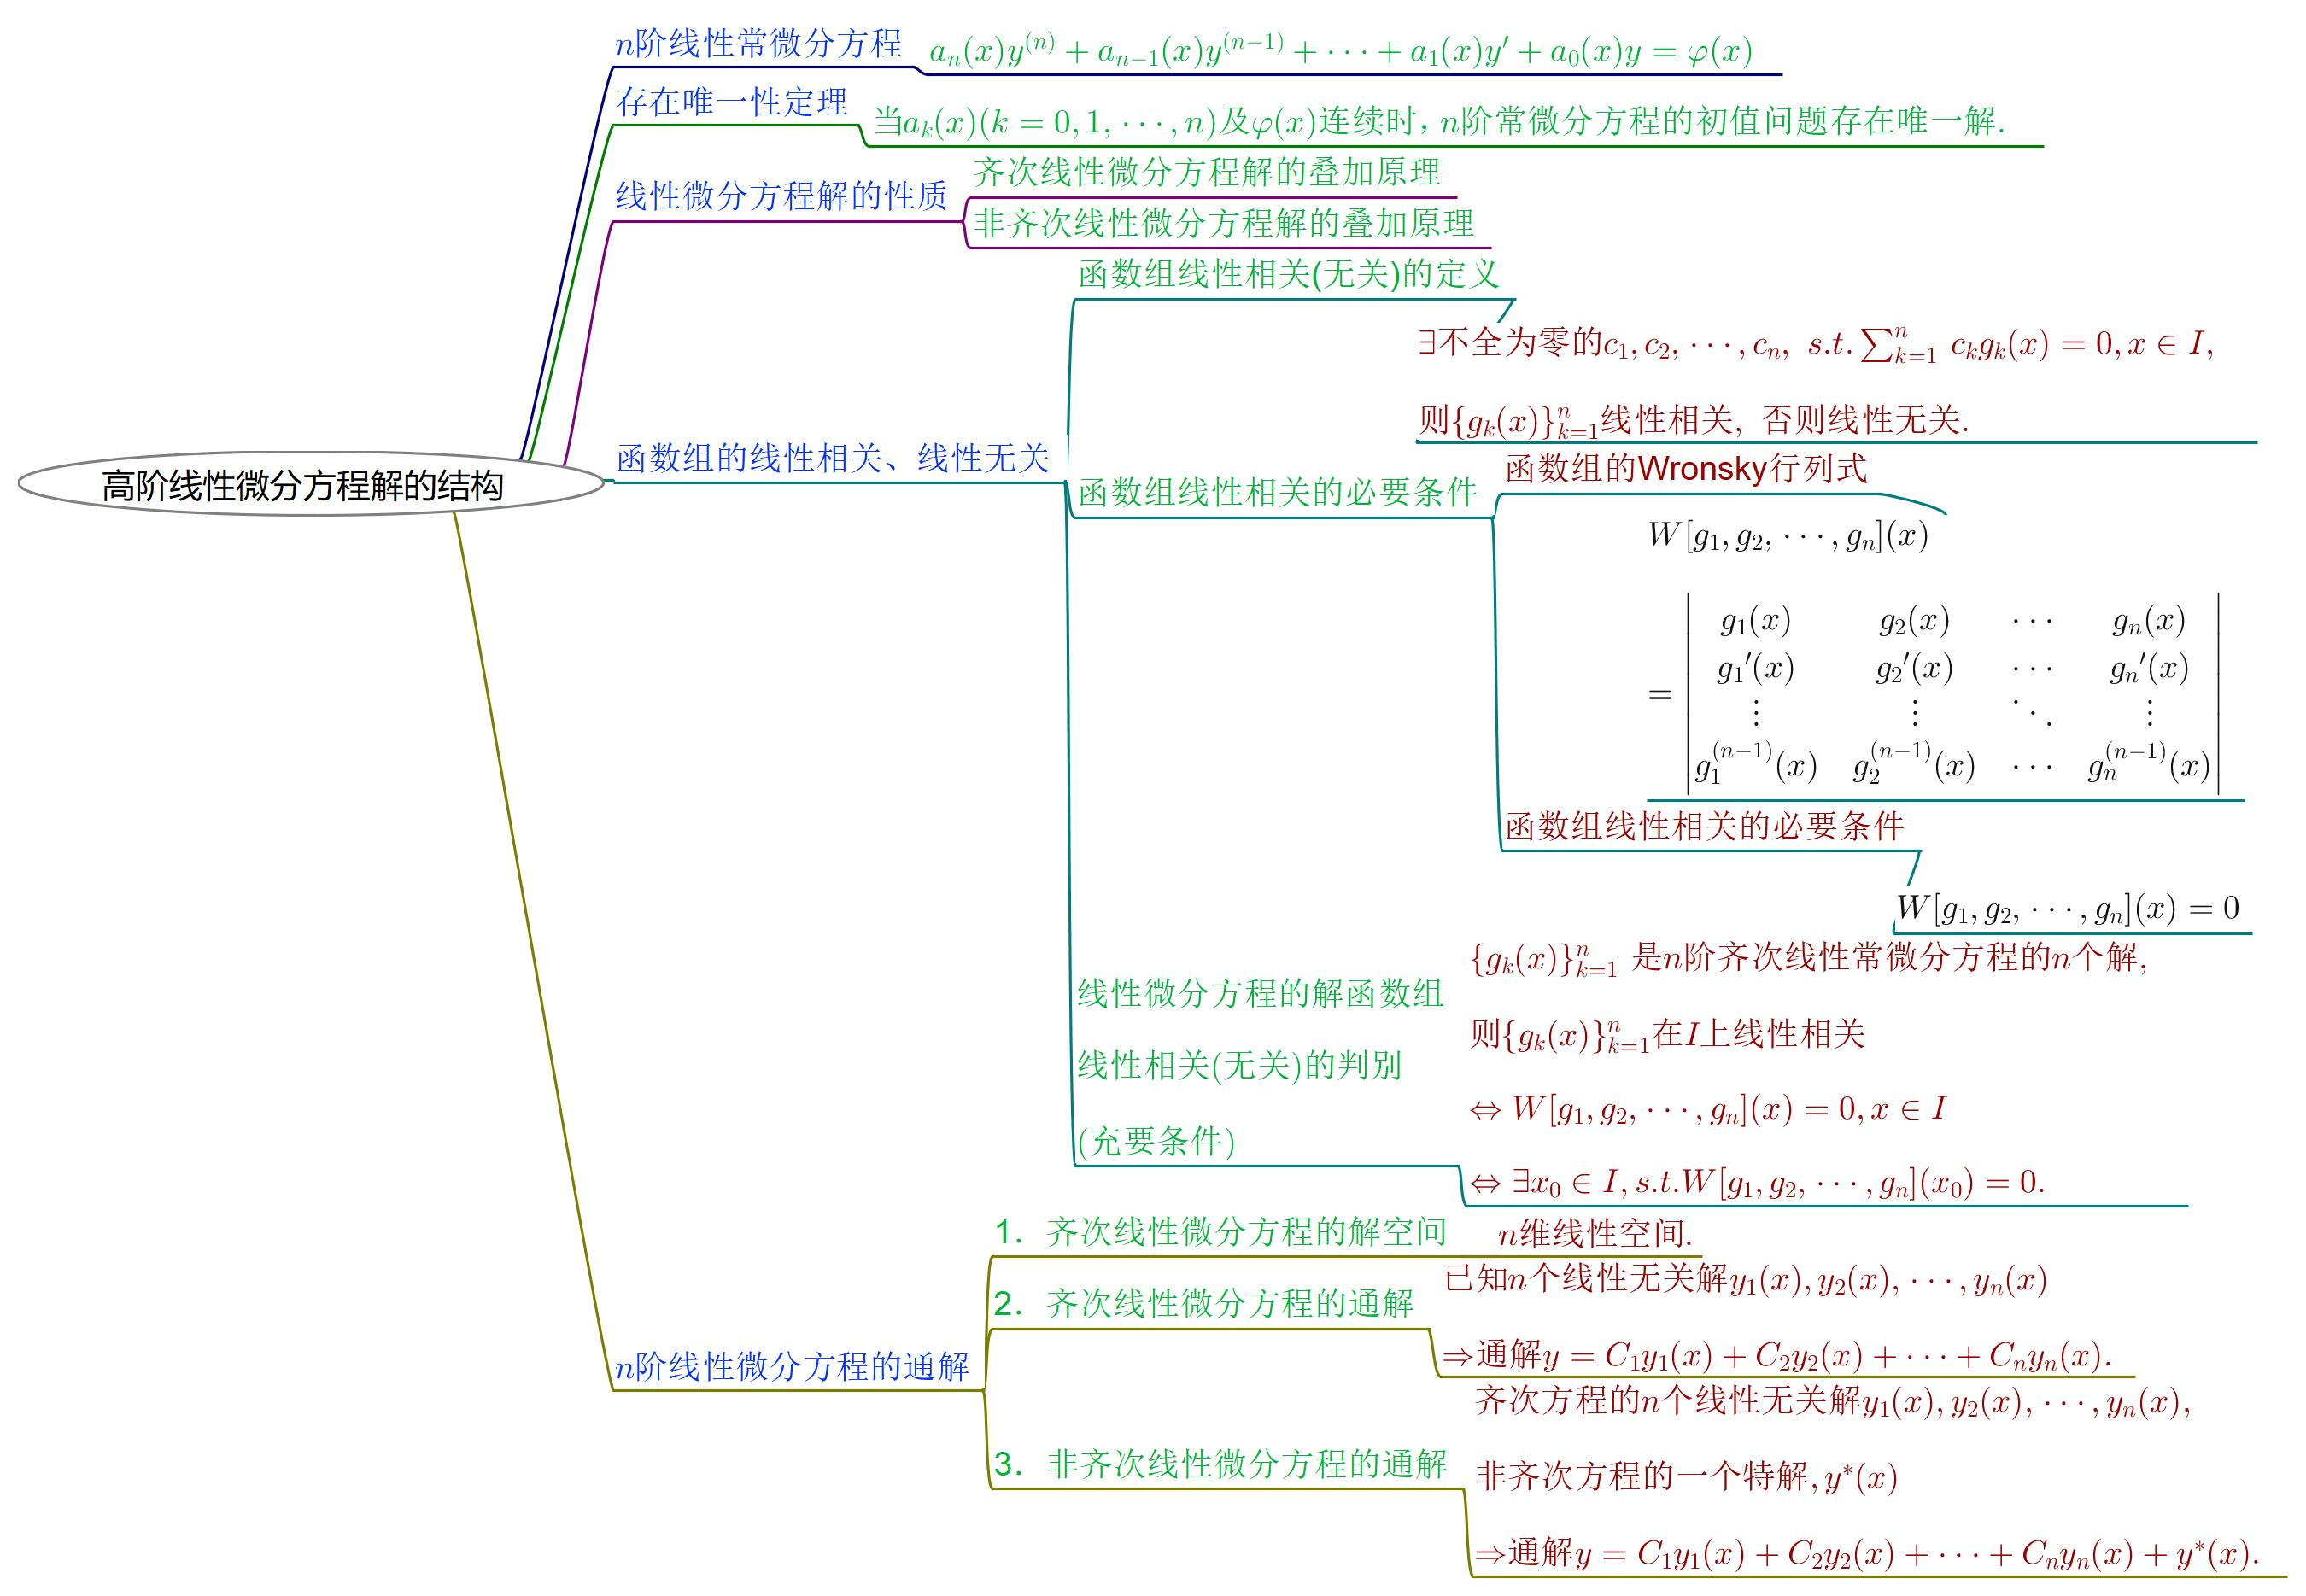
\includegraphics[height=0.5\textheight]{Figures27/Structures.jpg}
\end{center}
\end{figure}
\subsection{高阶线性常系数微分方程}
\begin{figure}[H]
\begin{center}
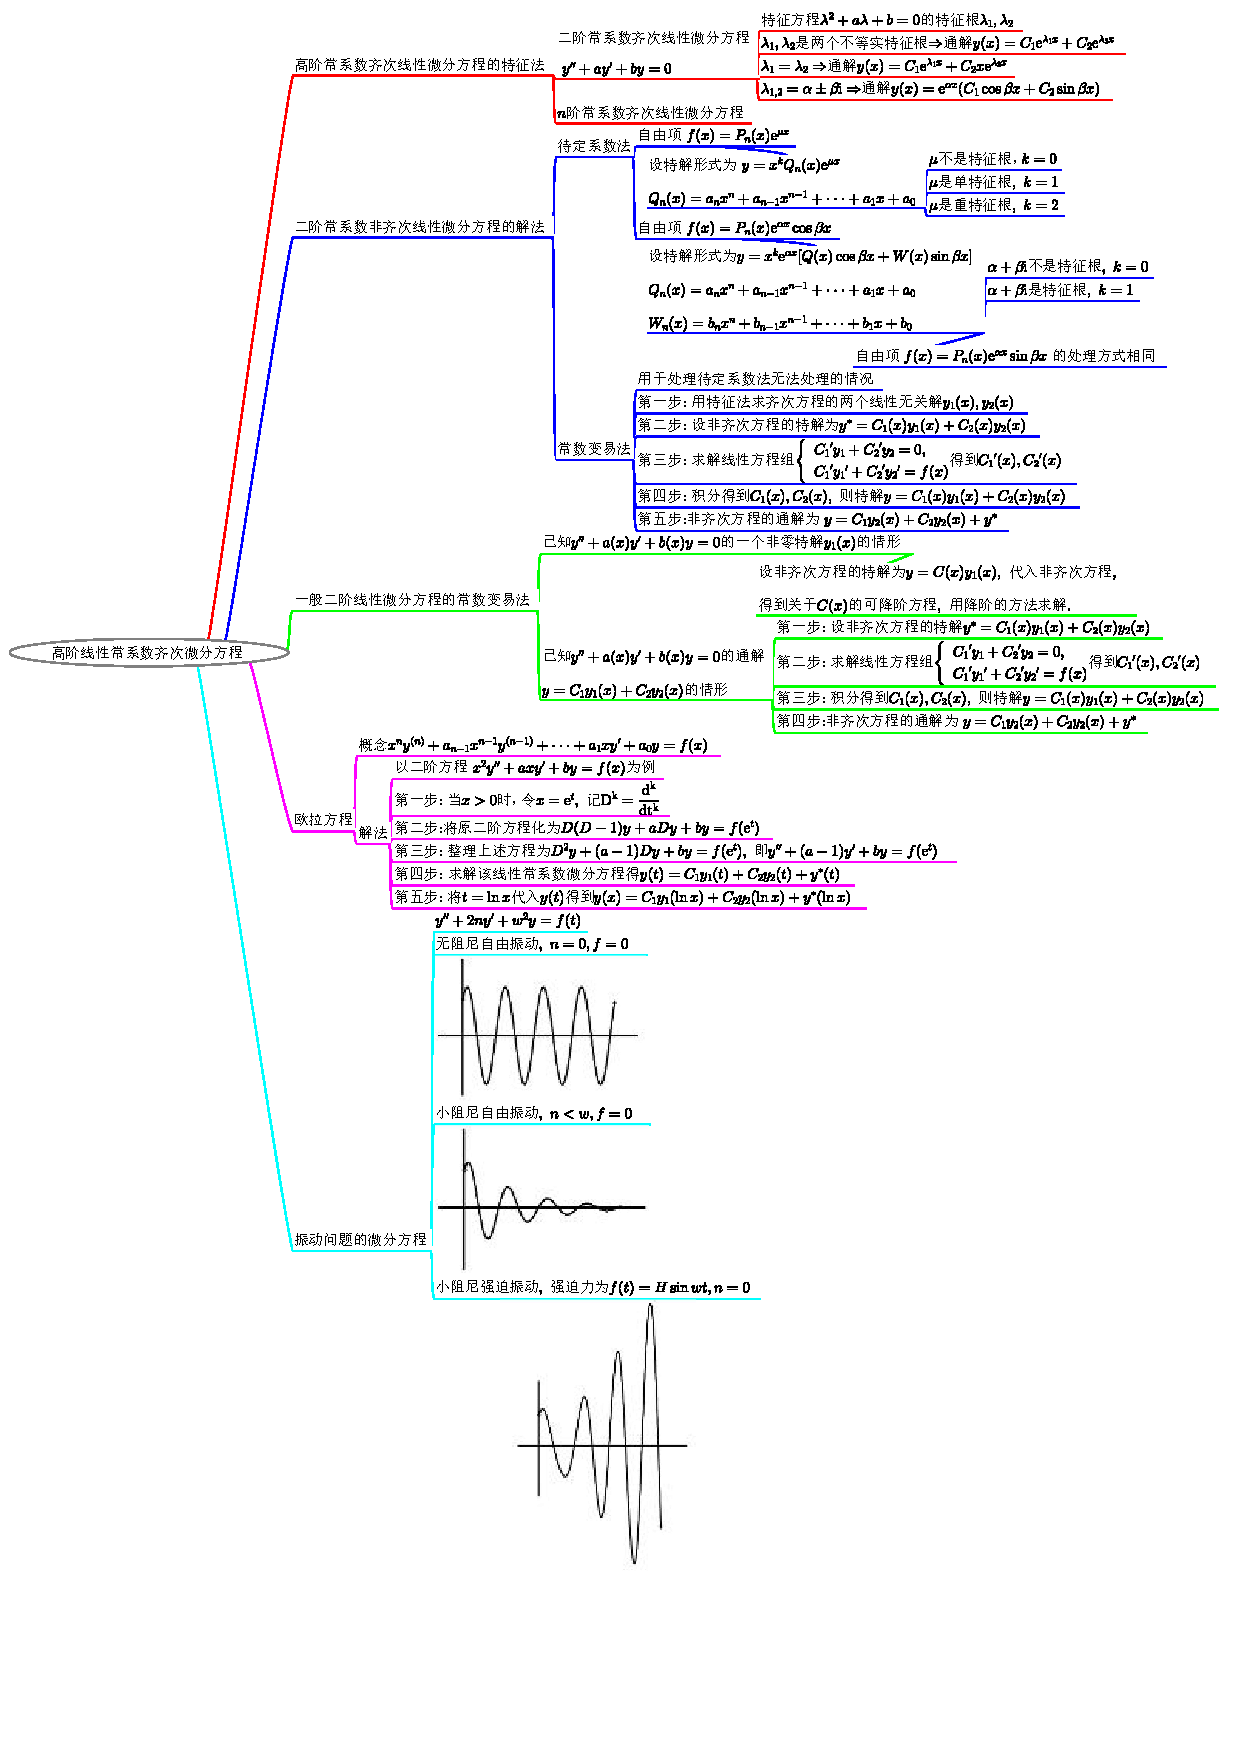
\includegraphics[height=1\textheight]{Figures27/Structures-2.pdf}
\end{center}
\end{figure}
\noindent【注意:】
\begin{enumerate}
\item求解二阶常系数非齐次线性微分方程首先判断自由项$f(x)$是否符合待定系数法可处理的两种形式之一,如符合,则采用待定系数法求解,如不符合则采用常数变易法求解.
\item已求得或已知二阶线性非齐次微分方程对应的齐次微分方程的通解$y=C_1y_1(x)+C_2y_2(x)$,利用常数变易法求非齐次方程的特解时,设特解为$y=C_1(x)y_1(x)+C_2(x)y_2(x)$之后,可直接求解线性方程组$\begin{cases}C_1'y_1+C_1'y_2=0,\\ C_1'y_1'+C_2'y_2'=f(x),\end{cases}$得到$C_1'(x)$和$C_2'(x)$,不需重新推导该方重组,直接代入该方程组求解即可.
\end{enumerate}
\subsection{习题分类与解题思路}
\subsubsection{高阶线性微分方程解的结构}
\begin{enumerate}
\item判断函数组在定义区间内是否线性相关. 可参考以下思路:
\begin{enumerate}
\item[第一步]计算Wronsky行列式. 若Wronsky行列式不恒等于零,则函数组线性无关.

【如习题14.3中的1.(1)/(2)/(3)/(4)/(5)/(6).】
\item[第二步]若Wronsky行列式恒等于零,则可按照线性相关的定义,判断是否存在不全为零的$c_1,c_2,\cdots,c_n\in\mathbb R$使得$\sum_{i=1}^nc_ng_n(x)=0$,若存在则线性相关,若不存在则线性无关.

若已知函数组是$n$阶线性微分方程的解函数组,则由Wronsky行列式恒等于零,可直接得到该函数组线性相关.
\end{enumerate}
\item考查齐次和非齐次线性方程解的叠加原理. 

【如习题14.3中的3.】
\item考查线性微分方程解的存在唯一性定理.

【如习题14.3中的6.】
\item考查$n$阶线性微分方程的解函数组线性相关(无关)判别的充要条件.

【如习题14.3中的7.】
\item考查$n$阶齐次线性微分方程解的结构. $n$阶齐次线性微分方程的解空间是$n$维线性空间,找到该齐次线性微分方程的$n$个线性无关的解,就可写出该齐次线性微分方程的通解.

【如习题14.3中的2.】
\item考查$n$阶非齐次线性微分方程解的结构. 先确定该非齐次方程对应的齐次方程的$n$个线性无关的解,从而求出齐次方程的通解,加上该非齐次方程的一个特解即可得到该非齐次方程的通解.

【如习题14.3中的8.】
\item其他类型的题目. 利用Wronsky行列式证明$n$阶非齐次线性微分方程有$n+1$个线性无关的解.

【如习题14.3中的9.】
\end{enumerate}
\subsubsection{高阶线性常系数微分方程}
\begin{enumerate}
\item求解齐次方程的通解. 利用特征法,要熟记三种特征根对应的通解形式. 求解思路为:
\begin{enumerate}
\item[第一步]列出特征方程,求出特征根.
\item[第二步]根据特征根写出齐次方程的通解.

注意二阶方程和二阶以上的方程不同特征根对应的齐次方程的通解的不同形式:
\begin{enumerate}
\item二阶方程:
\begin{itemize}
\item$\lambda_1\neq\lambda_2$是两个不等实特征根$\Rightarrow$通解$y=C_1\me^{\lambda_1x}+C_2\me^{\lambda_2x}$;
\item$\lambda_1=\lambda2$是一个二重根$\Rightarrow$通解$y=C_1\me^{\lambda_1x}+C_2x\me^{\lambda_2x}$;
\item$\lambda_{1,2}=\alpha\pm\beta\m i$为一对共轭复根$\Rightarrow$通解$y=\me^{\alpha x}(C_1\cos\beta x+C_2\sin\beta x)$.
\end{itemize}
\item二阶以上的方程:
\begin{itemize}
\item$\lambda$是特征方程的单重根$\Rightarrow y=\me^{\lambda x}$是一个特解;
\item$\lambda$是特征方程的$k$重根$\Rightarrow \me^{\lambda x},x\me^{\lambda x},\cdots,x^{k-1}\me^{\lambda x}$是$k$个线性无关的特解;
\item$\lambda=\alpha\pm\beta\m i$是特征方程的一对共轭复根$\Rightarrow\me^{\alpha x}\cos\beta x,\me^{\alpha x}\sin\beta x$是两个线性无关的解;
\item$\lambda=\alpha\pm\beta\m i$是特征方程的$k$对共轭复根\\
$\Rightarrow \me^{\alpha x}\cos\alpha x,x\me^{\alpha x}\cos\alpha x,\cdots,x^{k-1}\me^{\alpha x}\cos\alpha x,\\\me^{\alpha x}\sin\beta x,x\me^{\alpha x}\sin\beta x,\cdots,x^{k-1}\me^{\alpha x}\sin\beta x$.
\end{itemize}
$n$阶齐次方程按照以上方法得到的$n$个特解线性无关.
\end{enumerate}
\end{enumerate}

【习题14.4中的1.(1)/(2)/(3)/(4)/(5)/(6).】

注意其中的1.(4),要把特征方程左侧分解成最简因式的乘积,以判断特征根的重数.
\item给定常系数线性齐次微分方程的特解,求微分方程. 关键是根据特解的形式确定特征根,从而求出特征方程,根据特征方程写出齐次微分方程.

【习题14.4中的2.(1)/(2)/(3)/(4).】
\item写出二阶线性常系数非齐次方程的特解形式. 考查求非齐次方程特解的待定系数法. 
\begin{enumerate}
\item若自由项为$f(x)=P_n\me^{\mu x}$:
\begin{itemize}
\item当$\mu$不是特征根时,可设特解为$y=Q_n(x)\me^{\mu x}$;
\item当$\mu$是单特征根时,可设特解为$y=xQ_n(x)\me^{\mu x}$;
\item当$\mu$是重特征根时,可设特解为$y=x^2Q_n(x)\me^{\mu x}$;
\end{itemize}
其中$Q_n(x)=a_nx^n+a_{n-1}x^{n-1}+\cdots+a_1x+a_0$为一般形式的$n$次多项式.
\item若自由项为$f(x)=P_n\me^{\alpha x}\cos\beta x$或$f(x)=P_n\me^{\alpha x}\sin\beta x$:
\begin{itemize}
\item当$\alpha\pm\beta\m i$不是特征根时,可设特解为$y=\me^{\alpha x}[Q_n(x)\cos\beta x+W_n(x)\sin\beta x]$;
\item当$\alpha\pm\beta\m i$是共轭特征根时,可设特解为$y=x\me^{\alpha x}[Q_n(x)\cos\beta x+W_n(x)\sin\beta x]$.
\end{itemize}
其中$Q_n(x)=a_nx^n+a_{n-1}x^{n-1}+\cdots+a_1x+a_0, W_n(x)=b_nx^n+b_{n-1}x^{n-1}+\cdots+b_1x+b_0$为一般形式的$n$次多项式.

【习题14.4中的3.(1)/(2)/(3)/(4)/(5)/(6).】

对于含三角函数的自由项,可利用倍角公式、和差化积公式等化成待定系数法可处理的形式,如其中的3.(4)/(5).
\end{enumerate}
\item求解二阶常系数非齐次线性微分方程的解. 可参考以下步骤:
\begin{enumerate}
\item[第一步]写出对应齐次方程的特征方程,求出特征根,写出齐次方程的通解$y=C_1y_1(x)+C_2y_2(x)$;
\item[第二步]判断自由项$f(x)$是否为上述两种可用待定系数法处理的形式,若是,则用待定系数法求出非齐次方程的特解;

【如习题14.4中的4.(1)/(2)/(3)/(4)/(5).】
\item[第三步]若自由项$f(x)$不是上述可用待定系数法处理的形式之一,则用常数变易法求出非齐次方程的特解:
\begin{enumerate}
\item[第1步]设非齐次方程的特解为$y=C_1(x)y_1(x)+C_2(x)y_2(x)$;
\item[第2步]求解线性方程组$\begin{cases}C_1'y_1+C_2'y_2=0,\\C_1'y_1'+C_2'y_2'=f(x),\end{cases}$得到$C_1'(x),C_2'(x)$;
\item[第3步]积分$C_1'(x),C_2'(x)$得到$C_1(x)$和$C_2(x)$, 特解为$y=C_1(x)y_1(x)+C_2(x)y_2(x)$.
\end{enumerate}
注意:当已用特征法求出齐次方程的通解时,用常数变易法求特解只需代入第2步中的线性方程组求解$C_1'(x),C_2'(x)$,不需重新推导该方程.

【如习题14.3中的5.】
\item[第四步]若题目给定了初值条件,则代入初值条件,确定通解中的任意常数.

【如习题14.4中的6.】
\end{enumerate}
注意:题目中给定了初值条件时,应先求出非齐次方程的通解,用待定系数法或常数变易法求得的特解不一定满足初值条件.
\item考查欧拉方程. 可参考以下步骤(这里以二阶欧拉方程$x^2y''+axy'+by=f(x)$为例):
\begin{enumerate}
\item[第一步]当$x>0$时,令$x=\me^t$, 记$D^k=\frac{\md^k}{\md t^k}$;
\item[第二步]将欧拉方程中的$x^ky^{(k)}$用$D(D-1)\cdots(D-k+1)y$代换,自由项$f(x)$用$f(\me^t)$代换,得到线性常系数微分方程$D(D-1)y+aDy+by=f(\me^t)$, 整理成$D^2y+(a-1)Dy+by=f(\me^t)$即$y''+(a-1)y'+by=f(\me^t)$;
\item[第三步]求解该线性常系数微分方程,得到$y=C_1y_1(t)+C_2y_2(t)+y^*(t)$, 将$t$用$\ln x$代换,即可得到欧拉方程的通解$y=C_1y_1(\ln x)+C_2y_2(\ln x)+y^*(\ln x)$.
\end{enumerate}
考试时只需考虑$x>0$的情况. 当$x<0$时,令$x=-\me^t$,与$x>0$时仅有两点区别:
\begin{itemize}
\item一是最后得到的常系数微分方程的自由项变为$f(-\me^t)$, \\
方程形式为$D^2y+(a-1)Dy+by=f(-\me^t)$;
\item二是求得该线性常系数微分方程的通解后,应将$t$用$\ln(-x)$代换, \\
通解为$y=C_1y_1[\ln(-x)]+C_2y_2[\ln(-x)]+y^*[\ln(-x)]$.
\end{itemize}

【习题14.4中的6.(1)/(2).】
\item两个应用题大家可以积累一下.

【习题14.4中的7.(1)/(2).】
\end{enumerate}
\subsubsection{一般二阶线性微分方程的常数变易法}
\begin{enumerate}
\item给定$y''+a(x)y'+b(x)y=0$的非零特解$y_1(x)$时,可直接令非齐次方程$y''+a(x)y'+b(x)y=f(x)$的特解为$y=C(x)y_1(x)$,代入非齐次方程,得到关于$C(x)$的可降阶的二阶微分方程,解出$C(x)$,即可得到非齐次方程的一个特解$y=C(x)y_1(x)$.

【如习题14.3中的4.】

这里是用齐次方程的一个特解求该齐次方程的通解,而非求非齐次方程的特解,表明常数变易法是一个很强大的方法,也可以适用于已知齐次方程的特解,求该齐次方程的通解.
\item给定$y''+a(x)y'+b(x)y=0$的通解$y=C_1y_1(x)+C_2y_2(x)$,可按照以下步骤求非齐次方程$y''+a(x)y'+b(x)y=f(x)$的特解:
\begin{enumerate}
\item[第一步]设非齐次方程的一个特解为$y=C_1(x)y_1(x)+C_2(x)y_2(x)$;
\item[第二步]求解线性方程组$\begin{cases}C_1'y_1+C_2'y_2=0\\ C_1'y_1'+C_2'y_2'=f(x),\end{cases}$得到$C_1'(x),C_2'(x)$;
\item[第三步]积分$C_1'(x),C_2'(x)$得到$C_1(x),C_2(x)$,即可求出非齐次方程的特解$y=C_1(x)y_1(x)+C_2(x)y_2(x)$.
\end{enumerate}
这个过程与常系数非齐次线性微分方程的常数变易法相同. 这里也是直接求解第二步中的线性方程组得到$C_1'(x),C_2'(x)$,不需重新推导. 可参考常系数非齐次线性微分方程的常数变易法的这个题目:

【习题14.3中的5.】
\end{enumerate}
\subsection{习题14.3解答}
\begin{enumerate}
\item判断下列函数组在其定义区间内是否线性相关:\\
\begin{tabular}{ll}
(1)$1,x,x^2,x^3,x^4$;&(2)$\me^{-x},1,\me^x$;\\
(3)$\me^x,x\me^x$;&(4)$\sin x,\cos x$;\\
(5)$\me^x\cos x,\me^x\sin x$;&(6)$\ln x,x\ln x$.
\end{tabular}

解:(1)$W[1,x,x^2,x^3,x^4](x)=\begin{vmatrix}
1&x&x^2&x^3&x^4\\
0&1&2x&3x^2&4x^3\\
0&0&2&6x&12x^2\\
0&0&0&6&24x\\
0&0&0&0&24\\
\end{vmatrix}=1\cdot1\cdot2\cdot6\cdot24\not\equiv0$,

故$1,x,x^2,x^3,x^4$线性无关.

(2)$W[\me^{-x},1,\me^x](x)=\begin{vmatrix}
\me^{-x}&1&\me^x\\
-\me^{-x}&0&\me^x\\
\me^{-x}&0&\me^x
\end{vmatrix}=(-1)^3(-\me^{-x}\me^x-\me^x\me^{-x})=2\not\equiv0$,

故$\me^{-x},1,\me^x$线性无关.

(3)$W[\me^x,x\me^x](x)=\begin{vmatrix}
\me^x&x\me^x\\
\me^x&\me^x(x+1)
\end{vmatrix}=\me^{2x}(x+1)-x\me^{2x}=\me^{2x}\not\equiv0$,

故$\me^x,x\me^x$线性无关.

(4)$W[\sin x,\cos x](x)=\begin{vmatrix}\sin x&\cos x\\\cos x&-\sin x\end{vmatrix}=-1\not\equiv0$,

故$\sin x,\cos x$线性无关.

(5)$W[\me^x\cos x,\me^x\sin x](x)=\begin{vmatrix}
\me^x\cos x&\me^x\sin x\\
\me^x(\cos x-\sin x)&\me^x(\sin x+\cos x)\\
\end{vmatrix}=\me^x(\sin x\cos x+\cos^2x-\sin x\cos x+\sin^2x)=\me^x\not\equiv0$,

故$\me^x\cos x,\me^x\sin x$线性无关.

(6)$W[\ln x,x\ln x](x)=\begin{vmatrix}\ln x&x\ln x\\ \frac1x&\ln x+1\end{vmatrix}=(\ln x+1)\ln x-\ln x=(\ln x)^2\not\equiv0$,

故$\ln x,x\ln x$线性无关.

\item验证$y_1=\me^{x^2}$与$y_2=x\me^{x^2}$都是方程$y''-4xy'+(4x^2-2)y=0$的解,并写出该方程的通解.

解:$y_1=\me^{x^2},y_1'=\me^{x^2}2x,y_1''=2\me^{x^2}+4x^2\me^{x^2}$,

$y_1''-4xy_1'+(4x^2-2)y_1=2\me^{x^2}+4x^2\me^{x^2}-4x\me^{x^2}2x+(4x^2-2)\me^{x^2}=\me^{x^2}(2+4x^2-8x^2+4x^2-2)=0$,

$y_2=x\me^{x^2},y_2'=\me^{x^2}(1+2x^2),y_2''=\me^{x^2}(4x+2x+4x^3)=\me^{x^2}(6x+4x^3)$,

$y_2''-4xy_2'+(4x^2-2)y_2=\me^{x^2}(6x+4x^3)-4x\me^{x^2}(1+2x^2)+(4x^2-2)x\me^{x^2}\\
=\me^{x^2}(6x+4x^3-4x-8x^3+4x^3-2x)=0$,

$\therefore y_1,y_2$都是二阶线性齐次微分方程$y''-4xy'+(4x^2-2)y=0$的解.

$\because W[y_1,y_2](x)=\begin{vmatrix}\me^{x^2}&x\me^{x^2}\\2x\me^{x^2}&\me^{x^2}(1+2x^2)\end{vmatrix}=\me^{2x^2}(1+2x^2)-2x^2\me^{x^2}=\me^{x^2}\not\equiv0$,

$\therefore y_1,y_2$线性无关, 二阶线性齐次微分方程的通解为$y=C_1y_1+C_2y_2=C_1\me^{x^2}+C_2x\me^{x^2}$.

\item验证$y=\frac1x(c_1\me^x+c_2\me^{-x})+\frac12\me^x$($c_1,c_2$是任意常数)是方程$xy''+2y'-xy=\me^x$的通解.

解:$y_1=\frac1x\me^x,y_1'=\frac{\me^x(x-1)}{x^2},y_1''=\frac{\me^x(x-1+1)x^2-\me^x(x-1)2x}{x^4}=\frac{\me^x(x^2-2x+2)}{x^3}$,

$xy_1''+2y_1'-xy_1=x\frac{\me^x(x^2-2x+2)}{x^3}+2\frac{\me^x(x-1)}{x^2}-x\frac1x\me^x=\frac{\me^x(x^2-2x+2+2x-2-x^2)}{x^2}=0$,

$y_2=\frac{\me^{-x}}x,y_2'=\frac{-\me^{-x}x-\me^{-x}}{x^2}=\frac{-\me^{-x}(x+1)}{x^2},y_2''=\frac{\me^{-x}(x+1-1)x^2+\me^{-x}(x+1)2x}{x^4}=\frac{\me^{-x}(x^2+2x+2)}{x^3}$,

$xy_2''+2y_2'-xy_2=x\frac{\me^{-x}(x^2+2x+2)}{x^3}+2\frac{-\me^{-x}(x+1)}{x^2}-x\frac{\me^{-x}}x=\frac{\me^{-x}(x^2+2x+2-2x-2-x^2)}{x^2}=0$,

$y_3=\frac12\me^x,y_3'=\frac12\me^x,y_3''=\frac12\me^x$,

$xy''+2y'-xy=(x+2-x)\frac12\me^x=\me^x$,

$\therefore$根据叠加定理$y=c_1y_1+c_2y_2+y_3=\frac1x(c_1\me^x+c_2\me^{-x})+\frac12\me^x$是方程$xy''+2y'-xy=\me^x$的通解.

\item已知$y_1(x)=\me^x$是齐次方程$(2x-1)y''-(2x+1)y'+2y=0$的一个解,求该方程的通解.

解:设$y=u(x)\me^x$是方程$(2x-1)y''-(2x+1)y'+2y=0$的解,

$y'=\me^x(u'+u),y''=\me^x(u''+2u'+u)$,

则$(2x-1)y''-(2x+1)y'+2y=(2x-1)\me^x(u''+2u'+u)-(2x+1)\me^x(u'+u)+2u\me^x\\
=\me^x[(2x-1)u''+(4x-2-2x-1)u']+[(2x-1)(\me^x)''-(2x+1)(\me^x)'+2\me^x]u\\
=\me^x[(2x-1)u''+(2x-3)u']=0$,

$\therefore(2x-1)u''+(2x-3)u'=0$,

令$p(x)=u'$,则$p'(x)=u''$,

$\therefore(2x-1)p'+(2x-3)p=0$(*),

当$p\not\equiv0$时$\frac{\md p}p=\frac{3-2x}{2x-1}\md x=(-1+\frac2{2x-1})\md x$,

$\therefore\ln|p|=-x+\ln|2x-1|+C$,

$\therefore p=\pm\me^C\me^{-x}(2x-1)$,

$\because p\equiv0$也满足(*)式,

$\therefore p=u'=C\me^{-x}(2x-1)$,

$\therefore u=\int C\me^{-x}(2x-1)\md x=-C\me^{-x}(2x-1)+2C\int\me^{-x}\md x=-C\me^{-x}(2x-1)-2C\me^{-x}+C_1\\
=C\me^{-x}(-2x+1-2)+C_1=C_2(2x+1)\me^{-x}+C_1$,

$\therefore$原方程的通解为$y=[C_2(2x+1)\me^{-x}+C_1]\me^x=C_1\me^x+C_2(2x+1)$.

\item已知$y_1(x)=\cos x,y_2(x)=\sin x$是齐次方程$y''+y=0$的两个解,求非齐次方程$y''+y=\sec x$的通解.

解:由1.(4)知$y_1(x),y_2(x)$线性无关,故齐次方程$y''+y=0$的通解为\\$y=C_1\cos x+C_2\sin x$,

设非齐次方程$y''+y=\sec x$的解为$y=C_1(x)\cos x+C_2(x)\sin x$,

根据常数变易法$\begin{cases}C_1'(x)\cos x+C_2'(x)\sin x=0,\\-C_1'(x)\sin x+C_2'(x)\cos x=\sec x\end{cases}$, 解得$\begin{cases}
C_1'(x)=\frac{-\tan x}{\cos^2x+\sin^2x}=-\tan x,\\
C_2'(x)=\frac1{\cos^2x+\sin^2x}=1,
\end{cases}$

$\therefore\begin{cases}
C_1(x)=-\int\tan x\md x=\ln|\cos x|+C_3,\\
C_2(x)=\int\md x=x+C_4,
\end{cases}$

$\therefore$非齐次方程$y''+y=\sec x$的通解为$y=(\ln|\cos x|)\cos x+x\sin x+C_3\cos x+C_4\sin x$.

\item设$y=\varphi(x)$是方程$y''+p(x)y'+q(x)y=0$的一个不恒等于零的解,其中$p(x),q(x)$为$[a,b]$上的连续函数. 求证不存在$x_0\in(a,b)$, 使得$\varphi(x_0)=\varphi'(x_0)=0$.

证明:假设$\exists x_0\in(a,b),s.t.\varphi(x_0)=\varphi'(x_0)=0$,

$\because y\equiv0$也满足$y(x_0)=y'(x_0)=0$,

$\therefore$根据存在唯一性定理$\varphi(x)\equiv0$, 矛盾, 故假设不成立.

$\therefore$不存在$x_0\in(a,b)$, 使得$\varphi(x_0)=\varphi'(x_0)=0$.

\item设$p(x),q(x),r(x)$是区间$I$上的连续函数,$y_1(x),y_2(x),y_3(x)$是方程\[y'''(x)+p(x)y''(x)+q(x)y'(x)+r(x)y(x)=0\]的三个线性无关解,问是否存在$x_0\in I$,使得$y_1(x_0)=y_2(x_0)=y_3(x_0)=0$, 并说明理由.

解:假设存在$x_0\in I$,使得$y_1(x_0)=y_2(x_0)=y_3(x_0)=0$,

则$W[y_1,y_2,y_3](x_0)=\begin{vmatrix}y_1(x_0)&y_2(x_0)&y_3(x_0)\\ y_1'(x_0)&y_2'(x_0)&y_3'(x_0)\\y_1''(x_0)&y_2''(x_0)&y_3''(x_0)\end{vmatrix}=\begin{vmatrix}0&0&0\\ y_1'(x_0)&y_2'(x_0)&y_3'(x_0)\\y_1''(x_0)&y_2''(x_0)&y_3''(x_0)\end{vmatrix}=0$,

$\therefore$线性微分方程$y'''(x)+p(x)y''(x)+q(x)y'(x)+r(x)y(x)=0$的三个解$y_1(x),y_2(x),y_3(x)$线性相关,与题设矛盾,

$\therefore$不存在$x_0\in I$,使得$y_1(x_0)=y_2(x_0)=y_3(x_0)=0$.

\item设$y_1(x),y_2(x),y_3(x)$是方程\[y''(x)+p(x)y'(x)+q(x)y(x)=f(x)\]的三个特解,并且$\frac{y_2(x)-y_1(x)}{y_3(x)-y_1(x)}$不为常数. 求证$y(x)=(1-c_1-c_2)y_1(x)+c_1y_2(x)+c_2y_3(x)$是该方程的通解.

证明:$\because y_1(x),y_2(x),y_3(x)$是方程$y''(x)+p(x)y'(x)+q(x)y(x)=f(x)$的三个特解,

$\therefore$根据叠加定理$y_2(x)-y_1(x),\ y_3(x)-y_1(x)$是齐次方程$y''(x)+p(x)y'(x)+q(x)y(x)$的两个解, 

$\because\frac{y_2(x)-y_1(x)}{y_3(x)-y_1(x)}$不为常数,

$\therefore y_2(x)-y_1(x)$与$y_3(x)-y_1(x)$线性无关,

$\therefore$非齐次方程$y''(x)+p(x)y'(x)+q(x)y(x)=f(x)$的通解为
\[\begin{aligned}
y(x)&=c_1[y_2(x)-y_1(x)]+c_2[y_3(x)-y_1(x)]+y_1(x)\\
&=(1-c_1-c_2)y_1(x)+c_1y_2(x)+c_2y_3(x).
\end{aligned}\]
\item设函数$a_1(x),a_2(x),\cdots,a_n(x)$与$f(x)$连续,其中$f(x)\not\equiv0$,求证微分方程
\[y^{(n)}+a_1(x)y^{(n-1)}+\cdots+a_{n-1}(x)y'+a_n(x)y=f(x)\]
具有$n+1$个线性无关解,并用其$n+1$个线性无关解给出该方程的通解.

证明:设$\bar{y}_1(x),\bar{y}_2(x),\cdots,\bar{y}_n(x)$是齐次方程$y^{(n)}+a_1(x)y^{(n-1)}+\cdots+a_{n-1}(x)y'+a_n(x)y=0$的$n$个线性无关解,$\bar{y}$是非齐次方程$y^{(n)}+a_1(x)y^{(n-1)}+\cdots+a_{n-1}(x)y'+a_n(x)y=f(x)$的一个非零特解, 则$W[\bar y_1,\bar y_2,\cdots,\bar y_n](x)\not\equiv0$,

记$y_k(x)=\bar{y}_k(x)+\bar y(x),(k=1,2,\cdots,n)$, 则$y_k(x)$是非齐次方程的解,

则$W[y_1,y_2,\cdots,y_n,\bar y](x)\\
=W[\bar y_1,\bar y_2,\cdots,\bar y_n,\bar y](x)\\
=\begin{vmatrix}
\bar y_1(x)&\bar y_2(x)&\cdots&\bar y_n(x)&\bar y(x)\\
\bar y_1'(x)&\bar y_2'(x)&\cdots&\bar y_n'(x)&\bar y'(x)\\
\vdots&\vdots&\ddots&\vdots&\vdots\\
\bar y_1^{(n-1)}(x)&\bar y_2^{(n-1)}(x)&\cdots&y_{n}^{(n-1)}&\bar y^{(n-1)}(x)\\
\bar y_1^{(n)}(x)&\bar y_2^{(n)}(x)&\cdots&y_{n}^{(n)}&\bar y^{(n)}(x)
\end{vmatrix}$,

将该行列式的第$n-1$行$\times a_1(x)$,第$n-2$行$\times a_2(x),\cdots,$第$1$行$\times a_n(x)$加到第$n$行,考虑到$\bar y_k,k=1,2,\cdots,n$是齐次方程的解,$\bar y$是非齐次方程的解,得到

上式$=\begin{vmatrix}
\bar y_1(x)&\bar y_2(x)&\cdots&\bar y_n(x)&\bar y(x)\\
\bar y_1'(x)&\bar y_2'(x)&\cdots&\bar y_n'(x)&\bar y'(x)\\
\vdots&\vdots&\ddots&\vdots&\vdots\\
\bar y_1^{(n-1)}(x)&\bar y_2^{(n-1)}(x)&\cdots&y_{n}^{(n-1)}&\bar y^{(n-1)}(x)\\
0&0&\cdots&0&f(x)
\end{vmatrix}=f(x)W[\bar y_1,\bar y_2,\cdots,\bar y_n](x)\not\equiv0$,

$\therefore y_1(x),y_2(x),\cdots,y_n(x),\bar y(x)$线性无关,

故$y^{(n)}+a_1(x)y^{(n-1)}+\cdots+a_{n-1}(x)y'+a_n(x)y=f(x)$有$n+1$个线性无关解,

方程的通解为$y=C_1[y_1(x)-\bar y(x)]+C_2[y_2(x)-\bar y(x)]+\cdots+C_{n}[y_n(x)-\bar y(x)]+\bar y(x)$.
%设$c_1,c_2,\cdots,c_{n-1},c_n\in\mathbb R$,
%
%令
%\begin{equation}
%c_1y_1+c_2y_2+\cdots+c_{n-1}y_{n-1}+c_ny_n+c_{n+1}\bar y=0,
%\end{equation}
%
%将该式两边求$1$到$n$阶导数得
%\begin{subequations}
%\begin{equation}\tag{2}
%c_1y_1'+c_2y_2'+\cdots+c_{n-1}y_{n-1}'+c_ny_n'+c_{n+1}\bar y'=0,\end{equation}
%\begin{equation}\tag{3}
%c_1y_1''+c_2y_2''+\cdots+c_{n-1}y_{n-1}''+c_ny_n''+c_{n+1}\bar y''=0,
%\end{equation}
%\begin{equation}\notag
%\cdots,
%\end{equation}
%\begin{equation}
%\end{equation}
%\begin{equation}\tag{n}
%c_1y_1^{(n)}+c_2y_2^{(n)}+\cdots+c_{n-1}y_{n-1}^{(n)}+c_ny_n^{(n)}+c_{n+1}\bar y^{(n)}=0,
%\end{equation}
%\begin{equation}\tag{n+1}
%c_1y_1^{(n+1)}+c_2y_2^{(n+1)}+\cdots+c_{n-1}y_{n-1}^{(n+1)}+c_ny_n^{(n+1)}+c_{n+1}\bar y^{(n+1)}=0,
%\end{equation}
%\end{subequations}
%考虑到$y_1$$(1)+(2)\times a_1(x)+\cdots+(n-1)\times a_{n-1}+(n)\times a_n+(n+1)\times a_{n+1}$,

\end{enumerate}
\subsection{习题14.4解答}
\begin{enumerate}
\item求下列齐次方程的通解:\\
\begin{tabular}{ll}
(1)$y''+6y'+9y=0$;&(2)$y''+4y'+5y=0$;\\
(2)$y^{(4)}+y'''+y'+y=0$;&(4)$3y''-2y'-8y=0$;\\
(5)$y^{(6)}+2y^{(5)}+y^{(4)}=0$;&(6)$y'''+6y''+11y'+6y=0$.
\end{tabular}

解:(1)特征方程$\lambda^2+6\lambda+9=0$的根为$\lambda_{1,2}=-3$,

$\therefore$原方程的通解为$y=C_1\me^{-3x}+C_2x\me^{-3x}$.

(2)特征方程$\lambda^2+4\lambda+5=0$的根为$\lambda_{1,2}=\frac{-4\pm\sqrt{4^2-4\times5}}2=-2\pm\mathrm i$,

$\therefore$原方程的通解为$y=\me^{-2x}(C_1\cos x+C_2\sin x)$.

(3)特征方程$\lambda^4+\lambda^3+\lambda+1=(\lambda^3+1)(\lambda+1)=(\lambda+1)^2(\lambda^2-\lambda+1)=0$的根为\\
$\lambda_{1,2}=-1,\lambda_{3,4}=\frac{1\pm\sqrt{1-4\times1\times1}}2=\frac12\pm\frac{\sqrt 3}2\m i$,

$\therefore$原方程的解为$y=C_1\me^{-x}+C_2x\me^{-x}+\me^{\frac12x}[C_3\cos(\frac{\sqrt 3}2x)+C_4\sin(\frac{\sqrt 3}2x)]$.

(4)特征方程$3\lambda^2-2\lambda-8=(3\lambda+4)(\lambda-2)=0$的根为$\lambda_1=-\frac43,\lambda_2=2$,

$\therefore$原方程的解为$y=C_1\me^{-\frac43x}+C_2\me^{2x}$.

(5)特征方程$\lambda^6+2\lambda^5+\lambda^4=\lambda^4(\lambda+1)^2=0$的根为$\lambda_{1,2,3,4}=0,\lambda_{5,6}=-1$,

$\therefore$原方程的解为$y=C_1+C_2x+C_3x^2+C_4x^3+C_5\me^{-x}+C_6x\me^{-x}$.

(6)特征方程$\lambda^3+6\lambda^2+11\lambda+6=\lambda^3+6\lambda^2+9\lambda+2\lambda+6=\lambda(\lambda+3)^2+2(\lambda+3)\\
=(\lambda+3)[\lambda(\lambda+3)+2]=(\lambda+3)(\lambda^2+3\lambda+2)=(\lambda+3)(\lambda+2)(\lambda+1)=0$,

$\therefore$特征根为$\lambda_1=-1,\lambda_2=-2,\lambda_3=-3$,

$\therefore$原方程的解为$y=C_1\me^{-x}+C_2\me^{-2x}+C_3\me^{-3x}$.

\item求出以下列函数为特解的常系数线性齐次常微分方程:\\
(1)$\me^{2x},\me^{-2x}$,二阶;\\
(2)$\me^x,x\me^x$,二阶;\\
(3)$2,\cos x,\sin  x$,三阶;\\
(4)$\me^{-x},2x\me^{-x},3\me^x$,三阶.

解:(1)特征根为$\lambda_1=2,\lambda_2=-2$,特征方程为$(\lambda-2)(\lambda+2)=\lambda^2-4=0$,

$\therefore$齐次微分方程为$y''-4y=0$.

(2)特征根为$\lambda_{1,2}=1$,特征方程为$(\lambda-1)^2=\lambda^2-2\lambda+1=0$,

$\therefore$齐次微分方程为$y''-2y+y=0$.

(3)特征根为$\lambda_1=0,\lambda_{2,3}=\pm\m i$, 特征方程为$\lambda(\lambda^2+1)=\lambda^3+\lambda=0$,

$\therefore$齐次微分方程为$y'''+y'=0$.

(4)特征根为$\lambda_{1,2}=-1,\lambda=1$,特征方程为$(\lambda+1)^2(\lambda-1)=(\lambda^2+2\lambda+1)(\lambda-1)\\
=\lambda^3+2\lambda^2+\lambda-\lambda^2-2\lambda-1=\lambda^3+\lambda^2-\lambda-1=0$,

$\therefore$齐次微分方程为$y'''+y''-y'-y=0$.

\item写出下列非齐次方程的一个特解形式:\\
(1)$y''-5y'+6y=3\me^{4x}$;\\
(2)$y''+y=(x^2-1)\me^x$;\\
(3)$y''-2y'+5y=x\me^x\cos2x$;\\
(4)$y''+4y=2\cos^22x$;\\
(5)$y''+k^2y'=k\sin(kx+2)$;\\
(6)$y''+4y'+5y=\sin x$.

解:(1)该非齐次方程对应的齐次方程的特征方程$\lambda^2-5\lambda+6=(\lambda-2)(\lambda-3)=0$的根为$\lambda_1=2,\lambda_2=3$,

$\therefore$自由项$3\me^{4x}$中的$4$不是特征方程的根,

$\therefore$特解形式为$y=a\me^{4x}$.

(2)该非齐次方程对应的齐次方程的特征方程$\lambda^2+1=0$的特征根为$\lambda_{1,2}=\pm\m i$,

$\therefore$自由项$(x^2-1)\me^x$中的$1$不是特征方程的根,

$\therefore$特解形式为$y=(ax^2+bx+c)\me^x$.

(3)该非齐次方程对应的齐次方程的特征方程$\lambda^2-2\lambda+5=0$的根为$\lambda_{1,2}=\frac{2\pm\sqrt{4-4\times1\times5}}2=1\pm2\m i$,

$\therefore$自由项中的$1+2\m i$是特征方程的根,

$\therefore$特解形式为$y=x\me^x[(ax+b)\cos2x+(cx+d)\sin2x]$.

(4)$y''+4y=2\cos^22x=1+\cos4x$

方程$y''+4y=1$的自由项$1=\me^0$中的$0$不是特征方程$\lambda^2+4=0$的根,

方程$y''+4=\cos4x$的自由项$\cos4x$中的$4\m i$不是特征方程$\lambda^2+4=0$的根,

$\therefore$根据叠加原理,特解形式为$y=a+b\cos4x+c\sin4x$.

(5)自由项$k\sin(kx+2)=k\cos2\sin kx+k\sin2\cos kx$,

$\because k\m i$不是特征方程$\lambda^2+k^2\lambda=0$的根,

$\therefore$特解形式为$y=a\cos kx+b\sin kx$.

(6)设特解形式为$y=Q(x)\me^{0x}=Q(x)$, 代入原方程得$Q^{(4)}(x)-Q^{(3)}(x)=4$, 该方程左侧是与$Q^{(3)}$次数相同的多项式,为了使左右两侧的次数相同,故可设特解形式为$y=ax^3$.

\item求解下列二阶非齐次微分方程的解:\\
(1)$y''+2y'-3y=4x$;\\
(2)$2y''+y'-y=2\me^x$;\\
(3)$y''-3y'+2y=x\me^x$;\\
(4)$y''-3y'+2y=\cos x$;\\
(5)$y''+4y'+5y=\sin x$.

解:(1)特征方程$\lambda^2+2\lambda-3=(\lambda+3)(\lambda-1)=0$的特征根为$\lambda_1=-3,\lambda_1=1$,故齐次方程的通解为$y=C_1\me^{-3x}+C_2\me^x$,

$\because$非齐次方程的自由项为$4x=4x\me^0$, $\lambda=0$不是特征方程的解,

$\therefore$可设非齐次方程的特解为$y^*=ax+b$, 代入原非齐次方程得$0+2a-3ax-3b=4x$,

$\therefore -3a=4,2a-3b=0$,

$\therefore a=-\frac43,b=-\frac89$,

$\therefore$原非齐次方程的通解为$y=C_1\me^{-3x}+C_2\me^x-\frac43x-\frac89$.

(2)特征方程$2\lambda^2+\lambda-1=(2\lambda-1)(\lambda+1)=0$,

$\therefore$特征根$\lambda=\frac12,\lambda=-1$, 齐次方程的通解为$y=C_1\me^{\frac12x}+C_2\me^{-x}$,

$\because$原非齐次方程的自由项$\me^x$中的$\lambda=1$不是特征方程的根,

$\therefore$可设非齐次方程的特解为$y^*=a\me^x$,代入原特征方程得$2a\me^x+a\me^x-a\me^x=2\me^x$,

$\therefore a=1, y^*=\me^x$,

$\therefore$原非齐次方程的通解为$y=C_1\me^{\frac12x}+C_2\me^{-x}+\me^x$.

(3)特征方程$\lambda^2-3\lambda+2=(\lambda-1)(\lambda-2)=0$的根为$\lambda_1=1,\lambda_2=2$, 可知齐次方程的通解为$y=C_1\me^x+C_2\me^{2x}$,

$\because$原非齐次方程的自由项$x\me^x$中的$\lambda=1$是特征方程的解,

故可设非齐次方程的特解为$y^*=x(ax+b)\me^x$,

$\therefore {y^*}'=\me^x(ax^2+bx+2ax+b)=\me^x[ax^2+(2a+b)x+b],\\
{y^*}''=\me^x[ax^2+(2a+b)x+b+2ax+(2a+b)]=\me^x[ax^2+(4a+b)x+2a+2b]$, \\
代入原方程得$\me^x[ax^2+(4a+b)x+2a+2b-3ax^2-3(2a+b)x-3b+2ax^2+2bx]\\
=\me^x[(4a+b-6a-3b+2b)x+2a+2b-3b]=\me^x[-2ax+2a-b]=x\me^x$,

$\therefore -2a=1,2a-b=0$,

$\therefore a=-\frac12,b=-1$,

$\therefore {y^*}=x(-\frac12x-1)\me^x$,

$\therefore$原非齐次方程的通解为$y=C_1\me^x+C_2\me^{2x}-\frac12x(x+2)\me^x$.

(4)特征方程$\lambda^2-3\lambda+2=(\lambda-2)(\lambda-1)=0$的特征根为$\lambda_1=2,\lambda_2=1$, 故齐次方程的通解为$y=C_1\me^x+C_2\me^{2x}$,

$\because$非齐次方程的自由项$\cos x$中的$\lambda=\m i$是不是特征方程的根,

$\therefore$可设非齐次方程的特解为$y^*=a\cos x+b\sin x$,

$\therefore {y^*}'=-a\sin x+b\cos x, {y^*}''=-a\cos x-b\sin x$, 

代入原方程得$-a\cos x-b\sin x-3(-a\sin x+b\cos x)+2(a\cos x+b\sin x)=(-a-3b+2a)\cos x+(-b+3a+2b)\sin x=(a-3b)\cos x+(b+3a)\sin x=\cos x$,

$\therefore a-3b=1,b+3a=0$,

$\therefore a=\frac1{10},b=-\frac3{10},y^*=\frac1{10}(\cos x-3\sin x)$,

$\therefore$原非齐次方程的通解为$y=C_1\me^x+C_2\me^{2x}+\frac1{10}(\cos x-3\sin x)$.

(5)特征方程$\lambda^2+4\lambda+5=0$的根为$\lambda_{1,2}=\frac{-4\pm\sqrt{16-4\times5}}2=-2\pm\m i$, 故齐次方程的通解为$y=\me^{-2x}(C_1\cos x+C_2\sin x)$,

$\because$非齐次方程的自由项$\sin x$中的$\lambda=\m i$不是特征方程的根,

$\therefore$可设非齐次方程的特解为$y^*=a\cos x+b\sin x$,

${y^*}'=-a\sin x+b\cos x,{y^*}''=-a\cos x-b\sin x$,

代入原非齐次方程得$-a\cos x-b\sin x+4(-a\sin x+b\cos x)+5(a\cos x+b\sin x)=(-a+4b+5a)\cos x+(-b-4a+5b)\sin x=(4a+4b)\cos x+(-4a+4b)\sin x=\sin x$,

$\therefore 4a+4b=0,-4a+4b=1$,

$\therefore a=-\frac18,b=\frac18,y^*=-\frac18\cos x+\frac18\sin x$,

$\therefore$原非齐次方程的通解为$y=\me^{-2x}(C_1\cos x+C_2\sin x)-\frac18\cos x+\frac18\sin x$.

\item求下列二阶非齐次微分方程满足初值条件的特解:\\
(1)$y''+3y'+2y=\sin x,y(0)=y'(0)=0$;\\
(2)$y''+y'=\frac12\cos x,y(0)=y'(0)=0$.

解:(1)齐次方程$\lambda^2+3\lambda+2=(\lambda+2)(\lambda+1)=0$的根为$\lambda_1=-1,\lambda_2=-2$, 可知齐次方程的通解为$y=C_1\me^{-x}+C_2\me^{-2x}$,

该非齐次方程的自由项$\sin x$中$\lambda=\m i$不是特征方程的解, 故可设特解为$y=a\cos x+b\sin x$,

$y'=-a\sin x+b\cos x,y''=-a\cos x-b\sin x$,

代入原方程得$-a\cos x-b\sin x+3(-a\sin x+b\cos x)+2(a\cos x+b\sin x)=(-a+3b+2a)\cos x+(-b-3a+2b)\sin x=(a+3b)\cos x+(b-3a)\sin x=\sin x$,

$\therefore a+3b=0,b-3a=1$,

$\therefore a=-\frac3{10},b=\frac1{10}$, 特解为$y=-\frac3{10}\cos x+\frac1{10}\sin x$,

$\therefore$原非齐次方程的通解为$y=C_1\me^{-x}+C_2\me^{-2x}-\frac3{10}\cos x+\frac1{10}\sin x$,

$\because y(0)=C_1+C_2-\frac3{10}=0,y'(0)=-C_1-2C_2+\frac1{10}=0$,

$\therefore$满足初值条件的特解为$y(x)=\frac12\me^{-x}-\frac15\me^{-2x}-\frac3{10}\cos x+\frac1{10}\sin x$.

(2)特征方程$\lambda^2+\lambda=\lambda(\lambda+1)=0$的根为$\lambda_1=0,\lambda_2=-1$, 故齐次方程的通解为$y=C_1+C_2\me^{-x}$,

非齐次方程的自由项$\frac12\cos x$中的$\lambda=\m i$不是特征方程的根,故可设特解为$y=a\cos x+b\sin x$,

$y'=-a\sin x+b\cos x,y''=-a\cos x-b\sin x$,

代入原方程得$-a\cos x-b\sin x-a\sin x+b\cos x=(-a+b)\cos x+(-b-a)\sin x=\frac12\cos x$,

$\therefore a=-\frac14,b=\frac14$, 特解为$y=-\frac14\cos x+\frac14\sin x$,

故原方程的通解为$y=C_1+C_2\me^{-x}-\frac14\cos x+\frac14\sin x$,

$\because y(0)=C_1+C_2-\frac14,y'(0)=-C_2+\frac14=0$,

$\therefore C_1=0,C_2=\frac14$,

$\therefore$满足初值条件的特解为$\frac14\me^{-x}-\frac14\cos x+\frac14\sin x$.

\item求下列二阶微分方程的通解:\\
(1)$x^2y''+2xy'-2y=0$;\\
(2)$x^2y''+2xy'-2y=x^2+2$.

解:(1)当$x>0$时,令$x=\me^t$,则$t=\ln x$, 记$D^k=\frac{\md^k}{\md t^k}$,

则原方程可化为$D(D-1)y+2Dy-2y=0$, 即$(D^2+D-2)y=\frac{\md^2y}{\md t^2}+\frac{\md y}{\md t}-2y=0$,

特征方程$\lambda^2+\lambda-2=(\lambda+2)(\lambda-1)=0$的根为$\lambda_1=1,\lambda_2=-2$, 故$y=C_1\me^t+C_2\me^{-2t}$,

$\therefore$原方程的通解为$y=C_1x+\frac{C_2}{x^2},x>0$.

(2)当$x>0$时,令$x=\me^t$,则$t=\ln x$, 记$D^k=\frac{\md^k}{\md t^k}$, 则原方程可化为$D(D-1)y+2Dy-2y=\me^{2t}+2$,\\
即$(D^2+D-2)y=\frac{\md^2y}{\md t^2}+\frac{\md y}{\md t}-2y=\me^{2t}+2(*)$,

$\because$该方程自由项$\me^{2t}+2=\me^{2t}+2\me^{0t}$中的$\lambda=2$和$\lambda=0$都不是特征方程的根,

故可设特解为$y=a\me^{2t}+b,y'=2a\me^{2t},y''=4a\me^{2t}$,

代入方程$(*)$得$4a\me^{2t}+2a\me^{2t}-2a\me^{2t}-2b=4a\me^{2t}-2b=\me^{2t}+2$,

$\therefore 4a=1,-2b=2$,

$\therefore a=\frac14,b=-1$, 故特解为$y=\frac14\me^{2t}-1$,

$\because$方程$(*)$对应的齐次方程的通解为$y=C_1\me^t+C_2\me^{-2t}$,

$\therefore$方程$(*)$的通解为$y=C_1\me^t+C_2\me^{-2t}+\frac14\me^{2t}-1$,

$\therefore$原方程的通解为$y=C_1x+\frac{C_2}{x^2}+\frac14x^2-1,x>0$.

\item应用题:\\
(1)长度等于$6\text{m}$的链条在光滑桌面上滑动. 假定在开始时刻链条垂在桌面下的部分长度为$1\text{m}$,问链条全部滑下桌面需要多少时间?\\
(2)弹簧上端固定,下面挂有三个质量相同的重物,使弹簧伸长了$3a$. 若突然除去其中两个重物,弹簧开始自由振动,求重物的运动规律.

\begin{figure}[H]
\begin{center}
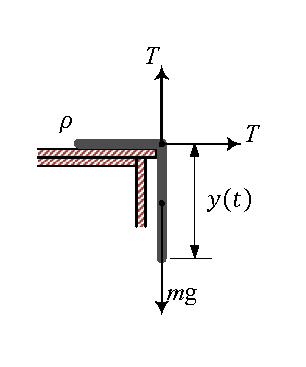
\includegraphics[height=0.5\textheight]{Figures27/14-4-7-2.pdf}
\end{center}
\caption{习题14.4 7.(1)题图示}
\end{figure}

解:(1)设$t$时刻链条垂下桌面的长度为$y=y(t)$,即$t$时刻,链条下端与桌面的垂直距离为$y(t)$,则$y(0)=1(\text{m}),y'(0)=0(\text{m/s})$,假设链条均匀,线密度为$\rho$,

则$t$时刻垂下桌面的部分的质量为$\rho y(t)$,桌面上的部分质量为$\rho[6-y(t)]$,

设垂下桌面的部分对桌面上的部分的拉力为$T$,

对于垂下桌面的部分,根据牛顿第二定律
\[\rho y(t)y''(t)=\rho y(t)\text{g}-T,\]
对于桌面上的部分,根据牛顿第二定律
\[\rho(6-y)y''(t)=T,\]
联立以上两个方程得
\[\rho y(t)y''(t)=\rho y(t)\text{g}-\rho(6-y)y'',\]
即
\[y''-\frac16\text{g}y=0,\]
该二阶齐次线性微分方程的特征方程为$\lambda^2-\frac16\text{g}=0$, 特征根为$\lambda_{1,2}=\pm\sqrt{\frac{\text{g}}6}$,

故该齐次线性微分方程的通解为$y=C_1\me^{-\sqrt{\frac{\text{g}}6}t}+C_2\me^{\sqrt{\frac{\text{g}}6}t}$,

$\because y(0)=C_1+C_2=1,y'(0)=-C_1\sqrt{\frac{\text{g}}6}+C_2\sqrt{\frac{\text{g}}6}=0$,

$\therefore C_1=C_2=\frac12$,

$\therefore y(t)=\frac12(\me^{-\sqrt{\frac{\text{g}}6}t}+\me^{\sqrt{\frac{\text{g}}6}t})=\cosh(\sqrt{\frac{\text{g}}6}t)$,

令$y(t)=6$得$\me^{\sqrt{\frac{\text{g}}6}t}=6+\sqrt{35}$或$6-\sqrt{35}$(小于1,故舍去),

$\therefore$链条全部滑下桌面用时$t=\sqrt{\frac6{\text g}}\ln(6+\sqrt{35})(\text{s})$.

\begin{figure}[H]
\begin{center}
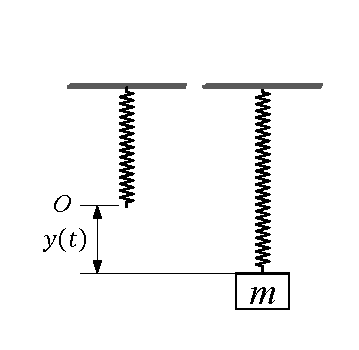
\includegraphics[height=0.5\textheight]{Figures27/14-4-7-1.pdf}
\end{center}
\caption{习题14.4 7.(2)题图示}
\end{figure}

(2)设弹簧常数为$k$,每个重物的质量为$m$,则$3m\m g=3ak$,即$m=\frac{ak}{\m g}$,

取弹簧未挂重物时的下端为坐标原点,设$t$时刻重物离开坐标原点的位移为$y(t)$,向下为正,则$y(0)=3a,y'(0)=0$,根据牛顿第二定律,
\[my''(t)=m\m g-ky(t),\]
即\[y''+\frac kmy=\m g,\]
因$m=\frac{ak}{\m g}$,故
\begin{equation}\label{14-4-7-2}y''+\frac{\m g}ay=\m g,\end{equation}
该二阶线性非齐次微分方程的齐次方程的特征方程为$\lambda^2+\frac{\m g}a=0$,特征根为$\lambda=\pm\sqrt{\frac{\m g}a}\m i$,

故齐次方程的通解为$y=C_1\cos(\sqrt{\frac{\m g}a}t)+C_2\sin(\sqrt{\frac{\m g}a}t)$,

非齐次方程~(\ref{14-4-7-2})的自由项$\m g=\m g\me^{0t}$中的$\lambda=0$不是特征方程的根,故可设非齐次方程的特解为$y=b$, 

代入方程~(\ref{14-4-7-2})得$0+\frac{\m g}ab=\m g$, 即$b=a$,

$\therefore$非齐次方程~(\ref{14-4-7-2})的通解为$y=C_1\cos(\sqrt{\frac{\m g}a}t)+C_2\sin(\sqrt{\frac{\m g}a}t)+a$,

$\because y(0)=C_1+a=3a,y'(0)=C_2\sqrt{\frac{\m g}a}=0$,

$\therefore C_1=2a,C_2=0$,

$\therefore$重物的运动规律为$y=2a\cos(\sqrt{\frac{\m g}a}t)+a$.
\end{enumerate}
\end{document}